% Created 2016-12-17 Sat 22:13
\documentclass[presentation]{beamer}
\usepackage[utf8]{inputenc}
\usepackage[T1]{fontenc}
\usepackage{fixltx2e}
\usepackage{graphicx}
\usepackage{longtable}
\usepackage{float}
\usepackage{wrapfig}
\usepackage{rotating}
\usepackage[normalem]{ulem}
\usepackage{amsmath}
\usepackage{textcomp}
\usepackage{marvosym}
\usepackage{wasysym}
\usepackage{amssymb}
\usepackage{hyperref}
\tolerance=1000
\usepackage[utf8]{inputenc}
\usetheme{diepen}
\author{Candace Makeda H. Moore, MD}
\date{\textit{<2016-12-11 Sun>}}
\title{Field Emergency App: Anamtastic}
\hypersetup{
  pdfkeywords={emergency medicine mobile app application},
  pdfsubject={Field Emergency App: Anamtastic},
  pdfcreator={Emacs 26.0.50.1 (Org mode 8.2.10)}}
\begin{document}

\maketitle
\begin{frame}{Outline}
\tableofcontents
\end{frame}


\section{Presentation}
\label{sec-1}
\subsection{Problems}
\label{sec-1-1}
\begin{frame}[label=sec-1-1-1]{Problems}
\begin{itemize}
\item Emergency care practitioners are under extreme time pressure
\item Significant portion of time taken for communication with  patient
\item Language barriers lengthen time and accuracy of information
\item Doctors are expected to remember all protocols
\item Doctors expected to remember all drugs, all side effect, all
interactions, all differential diagnoses, all lab values
\item These are unrealistic expectations which literally kill patients
\item Potential market for such apps is global
\end{itemize}
\end{frame}

\subsection{Solutions}
\label{sec-1-2}
\begin{frame}[label=sec-1-2-1]{Proposed}
\begin{itemize}
\item Anamastic is an app that addresses critical issues for patient
treatment and communication.
\item Anamtastic will be a multimodular app that the clinician can
tailor to her specific emergency setting
\end{itemize}
\end{frame}

\begin{frame}[label=sec-1-2-2]{Existing}
\begin{itemize}
\item Communication: right now translation in Israel is happening
ad-hoc based on a failing phone system from the MOH, google
translate and limited staff capabilities. If there was a better
tool we would all be using it.
\end{itemize}
\end{frame}

\subsection{Product Looks}
\label{sec-1-3}
\begin{frame}[label=sec-1-3-1]{Product Looks}
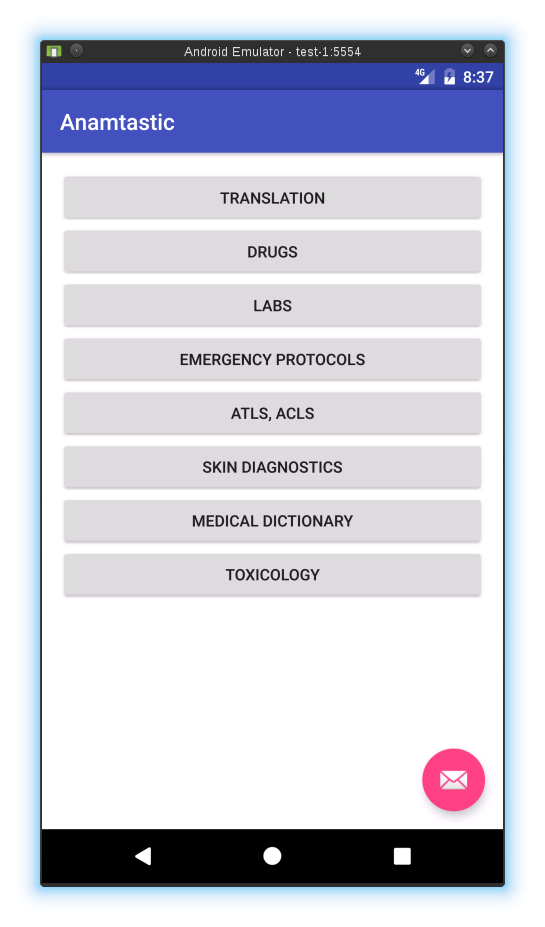
\includegraphics[width=3.6cm]{./presentation-images/module-selection-menu.png}
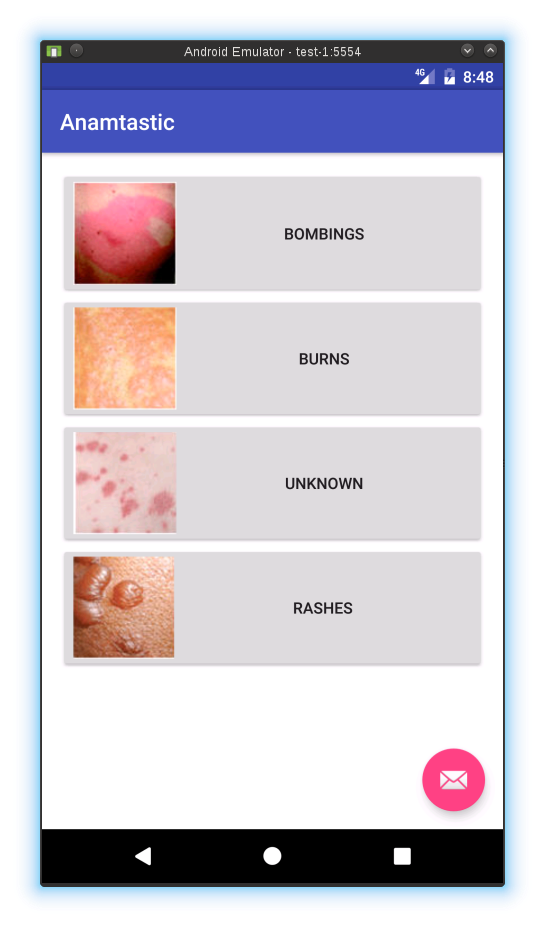
\includegraphics[width=3.6cm]{./presentation-images/skin-diagnostic-menu.png}
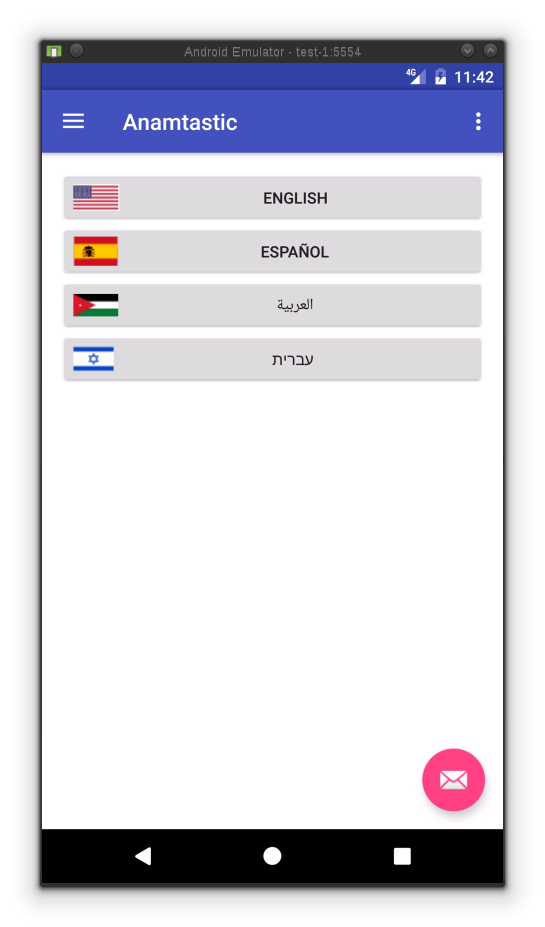
\includegraphics[width=3.6cm]{./presentation-images/language-select-menu.png}
\end{frame}

\subsection{App Market}
\label{sec-1-4}
\begin{frame}[label=sec-1-4-1]{App Market}
\begin{itemize}
\item Medical students, nurses, medics, physicians assistants and doctors
with smartphones
\item Nearly all doctors have smartphones--even in most African and Asian
countries
\item 3 billion a year market in USA alone
\item The market for such a product could be predicted by the performance
of similar yet inferior apps already on the market.  \alert{Epocrates} 50\%
penetrance of American physicians, revenues well over 500 million
each year for last three years.  \alert{PEPID} private company, low
penetrance, lack of reliable data on revenues
\item Mobile health app market is projected to hit 26 billion in revenue
by 2017
\end{itemize}
\end{frame}

\subsection{Costs And Plan}
\label{sec-1-5}
\begin{frame}[label=sec-1-5-1]{Building The First Modules}
\begin{itemize}
\item Staff salaries (3 programmers, one medical leader, one business
manager): 1,000,000 NIS, or \$250,000
\item Equipment (mobile phones, computers, additional cameras): 50,000
NIS
\item Expert consultations: 25,000 NIS
\item Workspace for meetings, food, other: 25,000 NIS
\item Total cost: 1,100,000 NIS or about \$300,000
\end{itemize}
\end{frame}

\begin{frame}[label=sec-1-5-2]{January 2017 Plan And Costs}
\begin{itemize}
\item Goal: Build prototype translation module and shell
\item Equipment (mobile phones, computers, additional cameras): 5,000
NIS
\item Expert consultations with front end designers: 25,000 NIS
\item Expert programmer with background as medic 5,000 NIS consult
\item Workspace for meetings, food, other: 5,000 NIS
\item Total cost: 40,000 NIS
\end{itemize}
\end{frame}

\subsection{Development Plan}
\label{sec-1-6}
\begin{frame}[label=sec-1-6-1]{Development Plan}
\begin{itemize}
\item Develop each module and release for sale separately to be put inside
the app shell which has one small free module (a compacted
translation phrasebook)
\item Development of translation module in first 3 months, release with
heavy marketing through Ministry of Health and Hospitals, post
release surveillance and improvement, and free partial phrasebook
\item Development of skin module next in parallel with development of
other modules that are closer to apps on the market i.e. medical
dictionary module, drug information and interaction model etc.
\item Exit strategy: At one year in case of incomplete funding: sell
existing modules to well funded companies or Ministry of Health
Israel, in case of good profitability: go public.
\end{itemize}
\end{frame}

\subsection{Team}
\label{sec-1-7}
\begin{frame}[label=sec-1-7-1]{Team}
\begin{columns}
\begin{column}{0.3\textwidth}
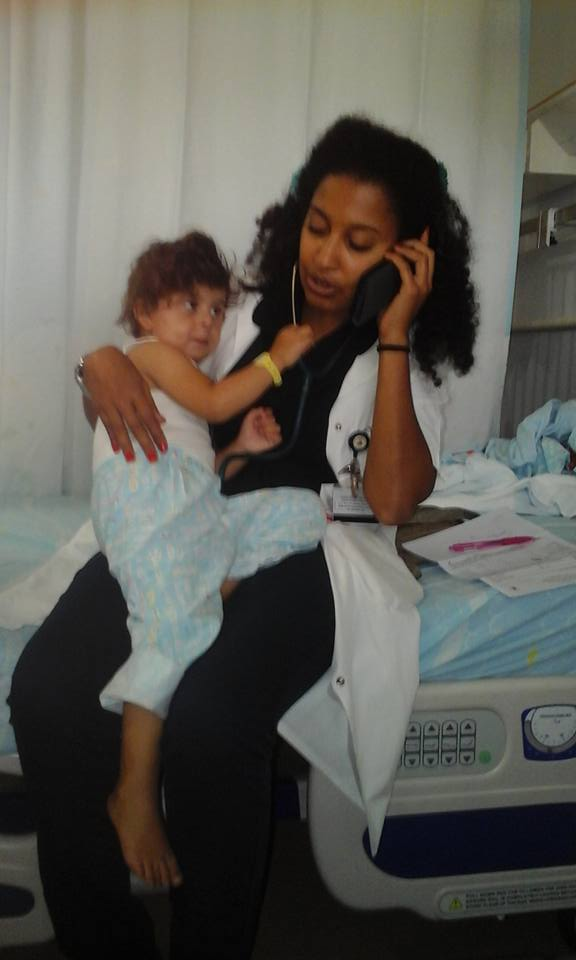
\includegraphics[width=3.0cm]{./presentation-images/makeda.jpeg}

Dr. Candace Makeda Moore, MD; (emergency doc, photographer,
founder)

\vspace{\fill}
\end{column}

\begin{column}{0.3\textwidth}
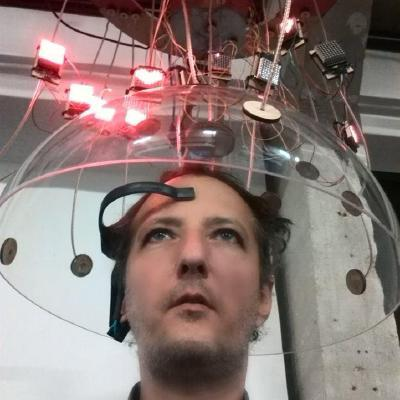
\includegraphics[width=3.0cm]{./presentation-images/jeremy-rutman.jpeg}

Dr. Jeremy Rutman, PhD, (patent attorney, computer
programmer/image pocessing, physicist)

\vspace{1.0cm}
\end{column}

\begin{column}{0.3\textwidth}
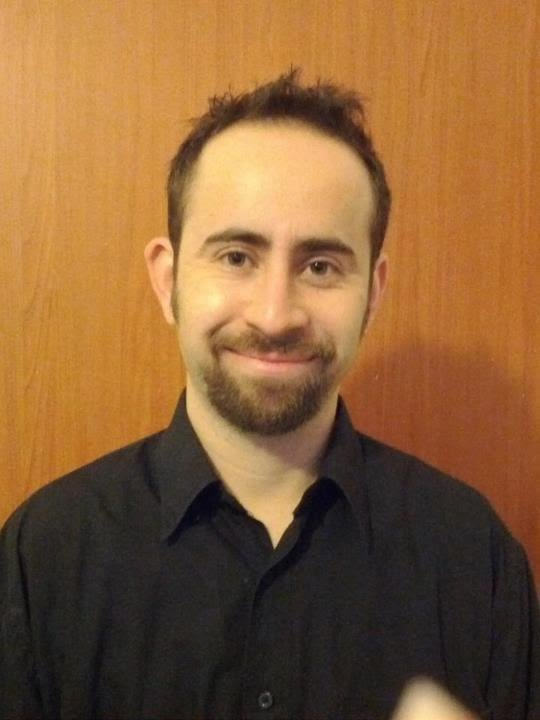
\includegraphics[width=3.0cm]{./presentation-images/mike-green.jpeg}

Mike Green, MS (biologist, computer programmer)

\vspace{2.0cm}
\end{column}
\end{columns}
\end{frame}

\subsection{Accomplishments}
\label{sec-1-8}
\begin{frame}[label=sec-1-8-1]{Accomplishments}
\begin{itemize}
\item Built website
\item Development of translation module underway, prototype/demo to be
completed on December 24$^{\text{th}}$, internal documents with algorithm and
design specifics currently in company dropbox
\item Collaboration with Trendiguru vis a vis Dr. Rutman to receive
algorithms for machine based 3D object recognition
\end{itemize}
\end{frame}

\subsection{The Real Plan}
\label{sec-1-9}
\begin{frame}[label=sec-1-9-1]{The Real Plan}
\begin{itemize}
\item As new modules are developed, starting with translation module
\item Try to sell modules to rivals i.e. PEPID, Epocrates, etc.
\item Try to push national acquisitions due to legal noncompliance
(providing care in patient's language mandated in some countries)
\item Business-wise we may be beat to market on some modules, but each can
be unpacked and sold once developed
\end{itemize}
\end{frame}
% Emacs 26.0.50.1 (Org mode 8.2.10)
\end{document}
